\documentclass[letterpaper,10pt]{extarticle}
\usepackage[utf8]{inputenc}
\usepackage[T1]{fontenc}
\usepackage{graphicx}
\usepackage[x11names]{xcolor}
\usepackage{tikz}
\usepackage[os=win]{menukeys}

\usepackage{amsmath,amssymb,textcomp}
\everymath{\displaystyle}

\usepackage{physics}

\usepackage{times}
\renewcommand\familydefault{\sfdefault}
\usepackage{tgheros}
\usepackage{droidmono}

\usepackage{enumitem}
\usepackage[explicit]{titlesec}

\usepackage{multicol}
\setlength{\columnseprule}{0pt}
\setlength{\columnsep}{15.0pt}

\usepackage{geometry}
\geometry{left=10mm,right=10mm,top=10mm,bottom=15mm}

% custom title
\makeatletter
\renewcommand*{\maketitle}{%
\noindent
\begin{minipage}{0.82\textwidth}

\begin{tikzpicture}
\node[rectangle,rounded corners=6pt,inner sep=6pt,fill=SteelBlue1,text width=.95\textwidth] {\color{black}\huge \@title};
\end{tikzpicture}
\end{minipage}
\hfill
\begin{minipage}{0.17\textwidth}
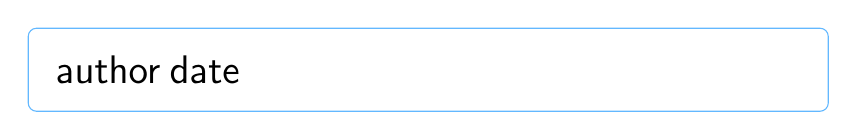
\begin{tikzpicture}
\node[rectangle,rounded corners=3pt,inner sep=10pt,draw=SteelBlue1,text width= 0.78\textwidth] {\raggedleft \Large \@author\ \@date};
\end{tikzpicture}
\end{minipage}
%\bigskip%\bigskip
}%
\makeatother

% custom section
\newcommand*\sectionlabel{}
\titleformat{\section}
  {\gdef\sectionlabel{}
   \normalfont\sffamily\Large\bfseries\scshape}
  {\gdef\sectionlabel{\thesection\ }}{0pt}
  {
\noindent
\begin{tikzpicture}
\node[rectangle,rounded corners=3pt,inner sep=4pt,fill=DodgerBlue4,text width= 0.95\columnwidth] {\color{white}\sectionlabel#1};
\end{tikzpicture}
  }
\titlespacing*{\section}{0pt}{.5pt}{0.5pt}

% custom subsection
\newcommand*\subsectionlabel{}
\titleformat{\subsection}{\normalfont\sffamily\bfseries\scshape}{\subsectionlabel}{0pt}{
\noindent
\begin{tikzpicture}
\node[rectangle,rounded corners=4pt,inner sep=3pt,fill=DodgerBlue3,text width= 0.95\columnwidth] {\color{white}\subsectionlabel#1};
\end{tikzpicture}
}
\titlespacing*{\subsection}{0pt}{.5pt}{.5pt}

% custom subsubsection
\newcommand*\subsubsectionlabel{}
\titleformat{\subsubsection}{\normalfont\sffamily\small\bfseries\scshape}{\subsubsectionlabel}{0pt}{
\noindent
\begin{tikzpicture}
\node[rectangle,rounded corners=3pt,inner sep=3pt,fill=blue!50!yellow,text width= 0.95\columnwidth] {\color{white}\subsubsectionlabel#1};
\end{tikzpicture}
}
\titlespacing*{\subsubsection}{0pt}{.5pt}{.5pt}


\title{MAT165 : Algèbre linéaire et analyse vectorielle}
\author{INTRA}
\date{A2018}

%\linespread{1.3}

\begin{document}
\maketitle

\begin{multicols*}{2}

\setlength{\belowdisplayskip}{2.5pt}
\setlength{\belowdisplayshortskip}{2.5pt}
\setlength{\abovedisplayskip}{2.5pt}
\setlength{\abovedisplayshortskip}{2.5pt}




\section{Vecteurs}
\vspace{-1.875\baselineskip}
Calculer un vecteur $\va{AB}$
\begin{align*}
    \va{AB} &= \qty[(b_1 - a_1),(b_2-a_2),(b_3-a_3)]\\
    &= \mathbf{vec}(\qty[a_1,a_2,a_3],\qty[b_1,b_2,b_3])
\end{align*}

\subsection{Norme d'un vecteur}
%\vspace{-1\baselineskip}
\begin{align*}
    \norm{\va{v}} &=\sqrt{(b_x-a_x)^2+(b_y-a_y)^2+(b_z-a_z)^2}\\
    &= \mathbf{norm}()
\end{align*}

\subsection{Vecteur unitaire}
%\vspace{-1\baselineskip}
\begin{equation*}
    \va{u} =\frac{\va{AB}}{\norm{\va{AB}}} = \mathbf{unitV}()
\end{equation*}

\section{Opérations sur les vecteurs}
\vspace{-2\baselineskip}
\subsection{Produit scalaire}
%\vspace{-1\baselineskip}
\begin{align*}
    \va{a} \cdot\va{b} &= \norm{\va{a}} \norm*{ \va{b} }\cos(\va{a} ~\angle ~ \va{b})\\
    &= \mathbf{dotP}()
\end{align*}\centering
\begin{tabular}{ll}
Angle aigu & \(\va{a} \cdot\va{b} > 0 \)\\
Angle obtu & \(\va{a} \cdot\va{b} < 0 \)\\
Angle droit & \(\va{a} \cdot\va{b} = 0 \)
\end{tabular}\\
\raggedright

\subsubsection{Angle entre deux vecteurs}
%\vspace{-1\baselineskip}
\centering
\begin{align*}
    \va{a} ~\angle~ \va{b} &= \arccos(\frac{\va{a}\cdot\vb{b}}{\norm{\va{a}}\norm*{\va{b}}})\\
    &= \mathbf{anglev}(\va{a},\va{b})
\end{align*}

\subsection{Produit vectoriel}
%\vspace{-1\baselineskip}
\begin{align*}
    \va{a} \wedge \va{b} &= \norm{\va{a}} \norm*{ \va{b} }\cos(\va{a}\wedge\va{b})\\
    &= \mathbf{crossP}()\\
    \mathit{Aire} &=  \norm*{\va{a} \cp \va{b}}
\end{align*}

\subsection{Produit mixte}
Le produit mixte est utile lorsque l'on veut calculer le volume.
\begin{align*}
    \mathit{Volume} &= \abs{\qty(\va{a} \cp\va{b}) \vdot \va{c}}\\
    &= \mathbf{vol}\qty(\va{a},\va{b},\va{c})
\end{align*}

\subsection{Composantes et projections}
%\vspace{-1\baselineskip}
\begin{align*}
    Comp_{\va{u}}\,\va{b} &= \frac{\va{a}\vdot\va{b}}{\norm{\va{a}}} = \va{u}\vdot \va{b} ,\; \va{u}=\frac{\va{a}}{\norm{\va{a}}}\\
    Proj_{\va{a}}\,\va{b} &= \frac{\va{a}\vdot\va{b}}{\norm{\va{a}}^2}\,\va{a} = \frac{\va{a}\vdot\va{b}}{\norm{\va{a}}}\frac{\va{a}}{\norm{\va{a}}}
\end{align*}

\section{Gradian}
%\vspace{-1\baselineskip}
\begin{align*}
    \grad{\va{f}}(x,y,z) &= \qty[\pdv{f}{x},\pdv{f}{y},\pdv{f}{z}]\\
    &= \mathbf{gradian}(var_{\mathit{list}},f,val_{\mathit{list}})
\end{align*}

\section{Courbes}
Une droite passant par le point $P(a_1,a_2,a_3)$
\subsubsection{Équations paramétriques vectorielle}
\begin{equation*}
    \va{r} = (a_1 + v_1 t)\va{i}+(a_2 + v_2 t)\va{j} +(a_3 + v_3 t)\va{k}
\end{equation*}

\subsubsection{Équations paramétriques scalaires}
    \begin{equation*} 
        f(x,y,z) = \left\{ 
            \begin{matrix}
            x &= a_1 + v_1 t\\
            y &= a_2 + v_2 t\\
            z &= a_3 + v_3 t
        \end{matrix}
        \right.
    \end{equation*}
    
\subsubsection{Équations symétriques}
% %\vspace{-1\baselineskip}
    \begin{equation*}
       \va{AP} // \va{v} \Leftrightarrow \frac{x-a_1}{v_1} = \frac{y-a_2}{v_2} = \frac{z-a_3}{v_3} \; \left| \begin{matrix} v_1 &\neq 0\\ v_2 &\neq 0\\ v_3 &\neq 0 \end{matrix} \right.
    \end{equation*}
    Exception: Si un des $v_1\neq0, v_2 = 0, v_3 \neq 0$

\subsection{Droite tangente}
\( \mathit{T_A} : \va{r}= \va{f}(t_a)+(t-t_a)\va{f}^\prime(t_a) \)

\subsection{Longueur d'arc}
%\vspace{-1\baselineskip}
\begin{align*}
    \overbrace{AB} &= \int^{t_b}_{t_a}\norm{\va{f}^\prime(t)}\dd{t}\\
     &= \mathbf{longarc}(v_{\mathrm{ind}},f,t_a,t_b)
\end{align*}

\subsection{Distance entre un point et une droite ($\va{QR}$)}
\begin{equation*}
    d = \frac{\norm{\va{PQ}\cp \va{v}}}{\norm{\va{v}}}
\end{equation*}

\subsection{Distance entre deux droites gauche}
\begin{equation*}
    d = \frac{\abs{\va{PQ}\vdot\qty(\va{v_1} \cp \va{v_2})}}{\norm{\va{v_1}\cp \va{v_2}}}
\end{equation*}

\section{Plans}
\subsection{Équation d'un plan}
\begin{align*}
    \Pi_A &: \va{N}\vdot\va{AP} = 0,\:A\qty(a_1,a_2,a_3)\; \mathrm{et}\; \va{N}=\qty(n_1,n_2,n_3)\\
    \Pi_A &: n_1\qty(x-a_1) + n_2\qty(y-a_2) + n_3\qty(z-a_3) = 0
\end{align*}

\subsection{Plan tangent}
\raggedright
Plan tangent passant par $P(a,b)$ membre de $f(a,b)$
\begin{equation*}
    \Pi_A : z = f(a,b) + f^\prime_x(a,b)(x-a) + f^\prime_y(a,b)(y-b)
\end{equation*}

\subsection{Vecteur normal}
%\vspace{-1\baselineskip}
\begin{align*}
% N_A &: \va{AP} // \grad{\va{f}}(a,b,c)\\
    f^\prime_{\va{u}} (a,b,c) &= \grad{\va{f}}(a,b,c)\va{u},\: \norm{\va{u}}=1 
\end{align*}
%\vspace{-1\baselineskip}
\begin{gather*}
    \underbrace{-\norm{\grad{\va{f}}\qty(a,b,c)}}_{\theta = \pi}\leq f^\prime_{\va{u}}\qty(a,b,c)\leq \underbrace{\norm{\grad{\va{f}}\qty(a,b,c)}}_{\theta = 0}
\end{gather*}

\subsection{Droite d'intersection de plans sécants}
\centering
\( v_1 = N_1 \cp N_2 \) est le vecteur directeur de la droite.

\subsection{Distance entre point et plan ou plan et plan}
\raggedright
\begin{equation*}
    distance = \frac{\abs{\va{PQ}\vdot\va{N}}}{\norm{\va{N}}}
\end{equation*}
Pour distance entre plans $//$, on choisi un point du plan $\Pi_2$

\subsection{Approximation linéaire}
% \centering
Approximer la fonction $f(x,y,z)$ au point $P(a,b,c)$
\begin{align*}
  %  f(x,y) &\approx f(a,b) + f^\prime_x(a,b)(x-a) + f^\prime_y(a,b)(y-b)\\
    f(x,y,z)\, &\approx f(a,b,c) + f^\prime_x(a,b,c)(x-a) + f^\prime_y(a,b,c)(y-b) \\ &\quad+ f^\prime_z(a,b,c)(z-c)
\end{align*}

\subsection{Approximation de l'erreur}
Erreur absolue:
\[ \Delta f(a,b,c) \approx f^\prime_x(a,b,c) \Delta x + f^\prime_y(a,b,c) \Delta y + f^\prime_z(a,b,c) \Delta z \]
Erreur relative: \[ \frac{\Delta f(a,b,c)}{f(a,b,c)}\]


\section{Optimisation}
\begin{enumerate}
    \item Variables décisionnelles: $x,y,z$
    \item Fonction économique: $f(x,y,z)$
    \item Contrainte: $g(x,y,z)=c$
\end{enumerate}%\vspace{-1\baselineskip}
\begin{gather*}
    \mathbf{lap21}\qty(x,y,f,g,c) \qq{} \mathbf{lap31}\qty(x,y,z,f,g,c)
\end{gather*}
\begin{enumerate}[nosep]
\setcounter{enumi}{3}
    \item Évaluer la fonction aux points trouvés afin de déterminer la nature du point (min/max).
\end{enumerate}


% \input{fonction_par_morceaux.tex}
% \input{laplace.tex}
% \input{series_puissances_sol_ed.tex}
% \input{series_fourier.tex}
% \input{prolongement_periodique.tex}



% %Applications
% \input{ressorts.tex}

% \input{runge-kutta.tex}
% 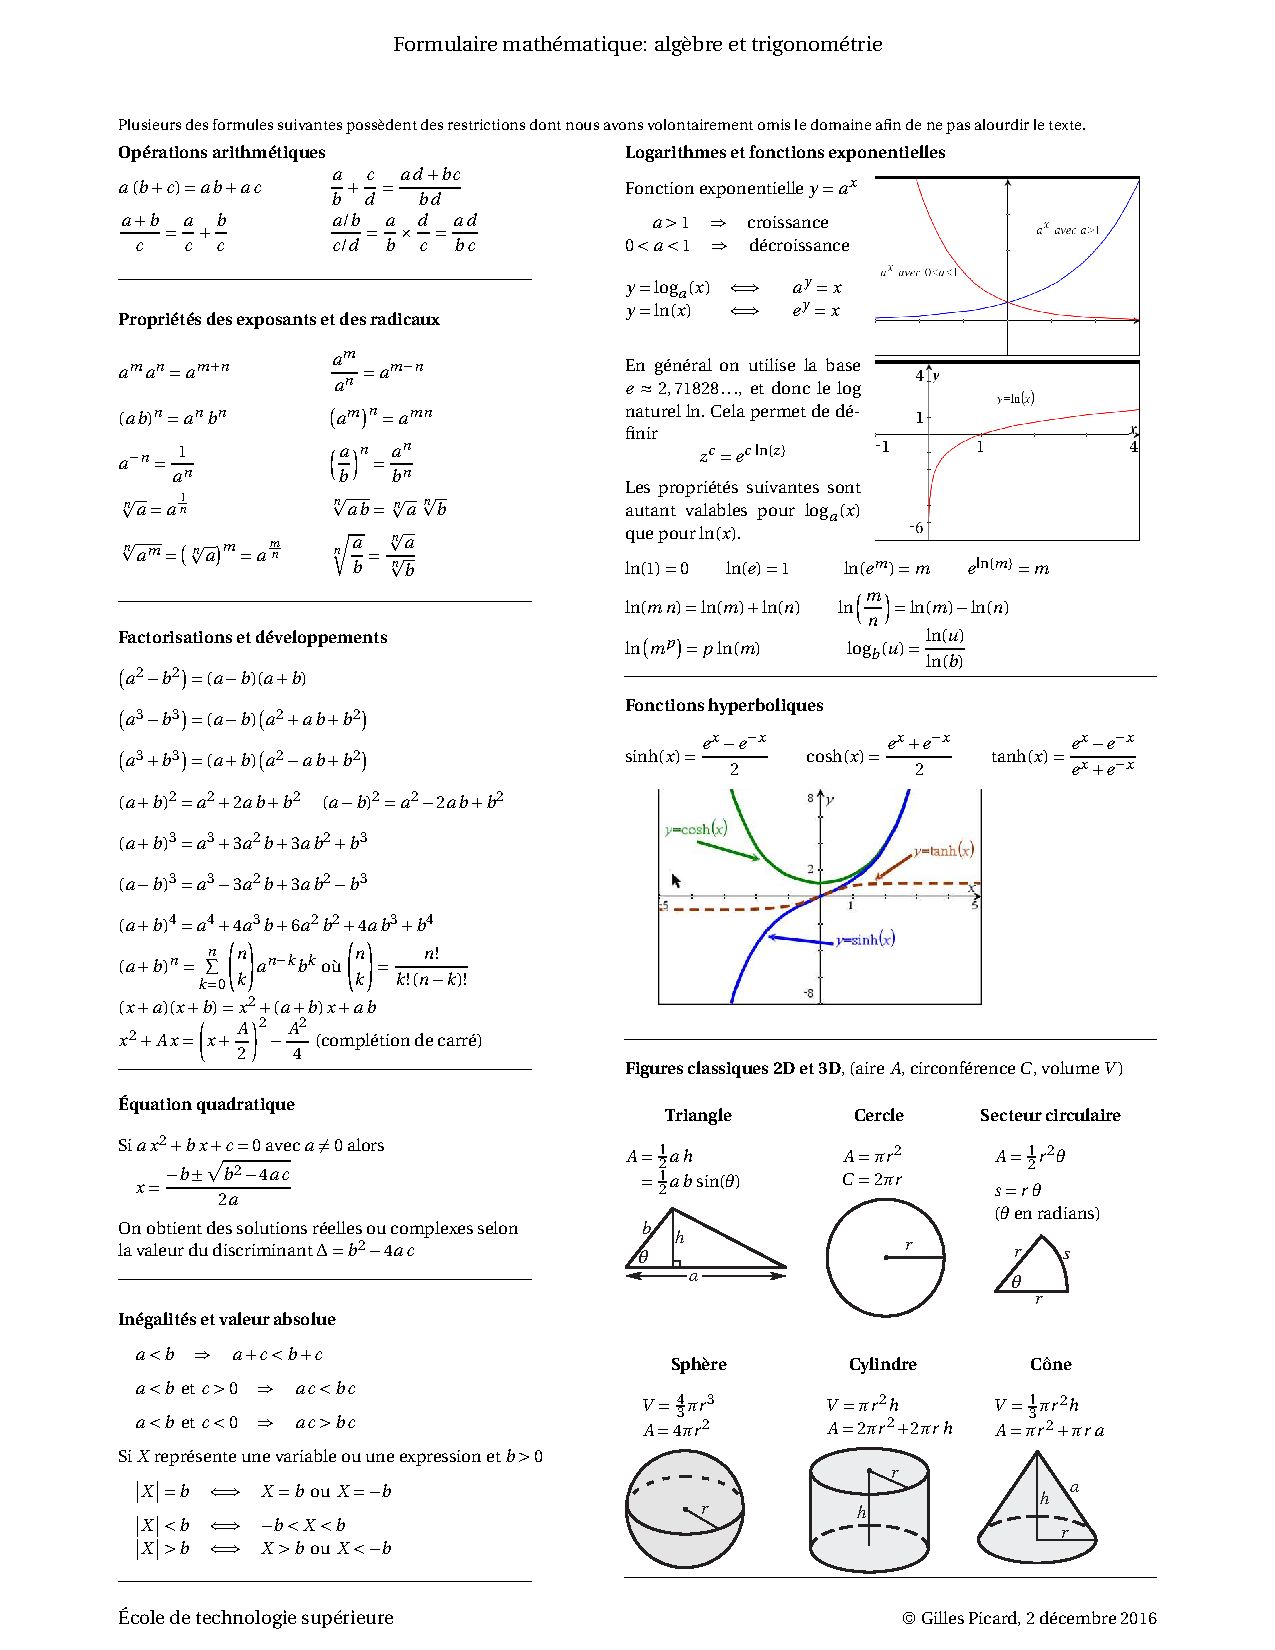
\includepdf[pages=-]{formulaire-algebre-trigo.pdf}


\end{multicols*}

\end{document}
